\documentclass[10pt]{beamer}
\usepackage[german]{babel}
\usepackage[utf8]{inputenc}
\usepackage{textgreek}


\title[soldering-workshop] % (optional, only for long titles)
{Lötworkshop @ PAM 10.5}
\author{Eileen, towa}
\usetheme{metropolis}

\begin{document}
    \maketitle

    \begin{frame}
        \frametitle{Lötkolben}
        \begin{itemize}
            \item{Temperaturen: 200 - 450 Grad Celsius.}
            \item{Lötspitzen sind beschichtet.}
            \item{Es sollte immer ein wenig Zinn an der Lötspitze sein.}
        \end{itemize}
    \end{frame}

    \begin{frame}
        \frametitle{Lot}
        \begin{itemize}
            \item{Blei- und Silberhaltiges Lot.}
            \item{Flußmittelseele im Lot enthalten.}
            \item{Flußmittel verbessert Flußeigenschaften des Zinns.}
        \end{itemize}
        \begin{figure}[hbtp]
            \centering
            
\includegraphics[width=\linewidth]{images/lotseele.png}
            \caption{Quelle: ERSA Lötfibel}
        \end{figure}
    \end{frame}

    \begin{frame}
        \frametitle{Lötvorgang}
            \begin{columns}[T] % align columns
                \begin{column}{.33\textwidth}
                    \textbf{Benetzen} \newline
                    Auf die gereinigte Lötspitze etwas Lot geben.
                \end{column}%
                \hfill%
                \begin{column}{.33\textwidth}
                    \textbf{Fließen} \newline
                    Die Lötstelle erhitzen und soviel Lot dazu geben wie nötig.
                \end{column}%
                \begin{column}{.33\textwidth}
                    \textbf{Binden} \newline
                    Erst Lot, dann Spitze von Lötstelle entfernen und anschließen abkühlen lassen.
                \end{column}%
                \hfill%
            \end{columns}
    \end{frame}

    \begin{frame}
        \frametitle{Löten 101}
        \begin{figure}[hbtp]
            \centering
            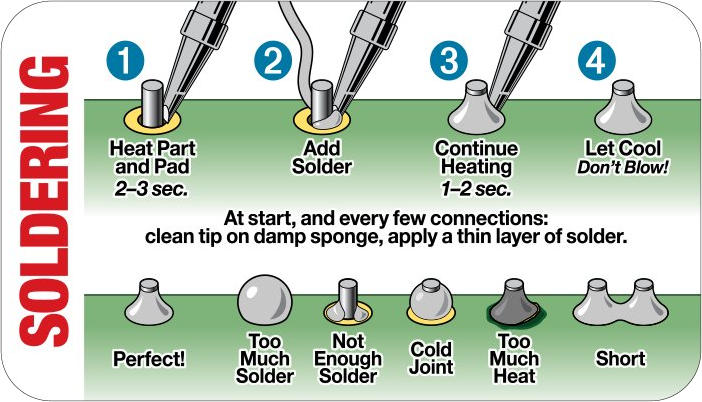
\includegraphics[width=\linewidth]{images/solder.png}
            \caption{Quelle: Adafruit}
        \end{figure}
    \end{frame}


    \begin{frame}
        \frametitle{Das Badge}
        \begin{figure}[hbtp]
            \centering
            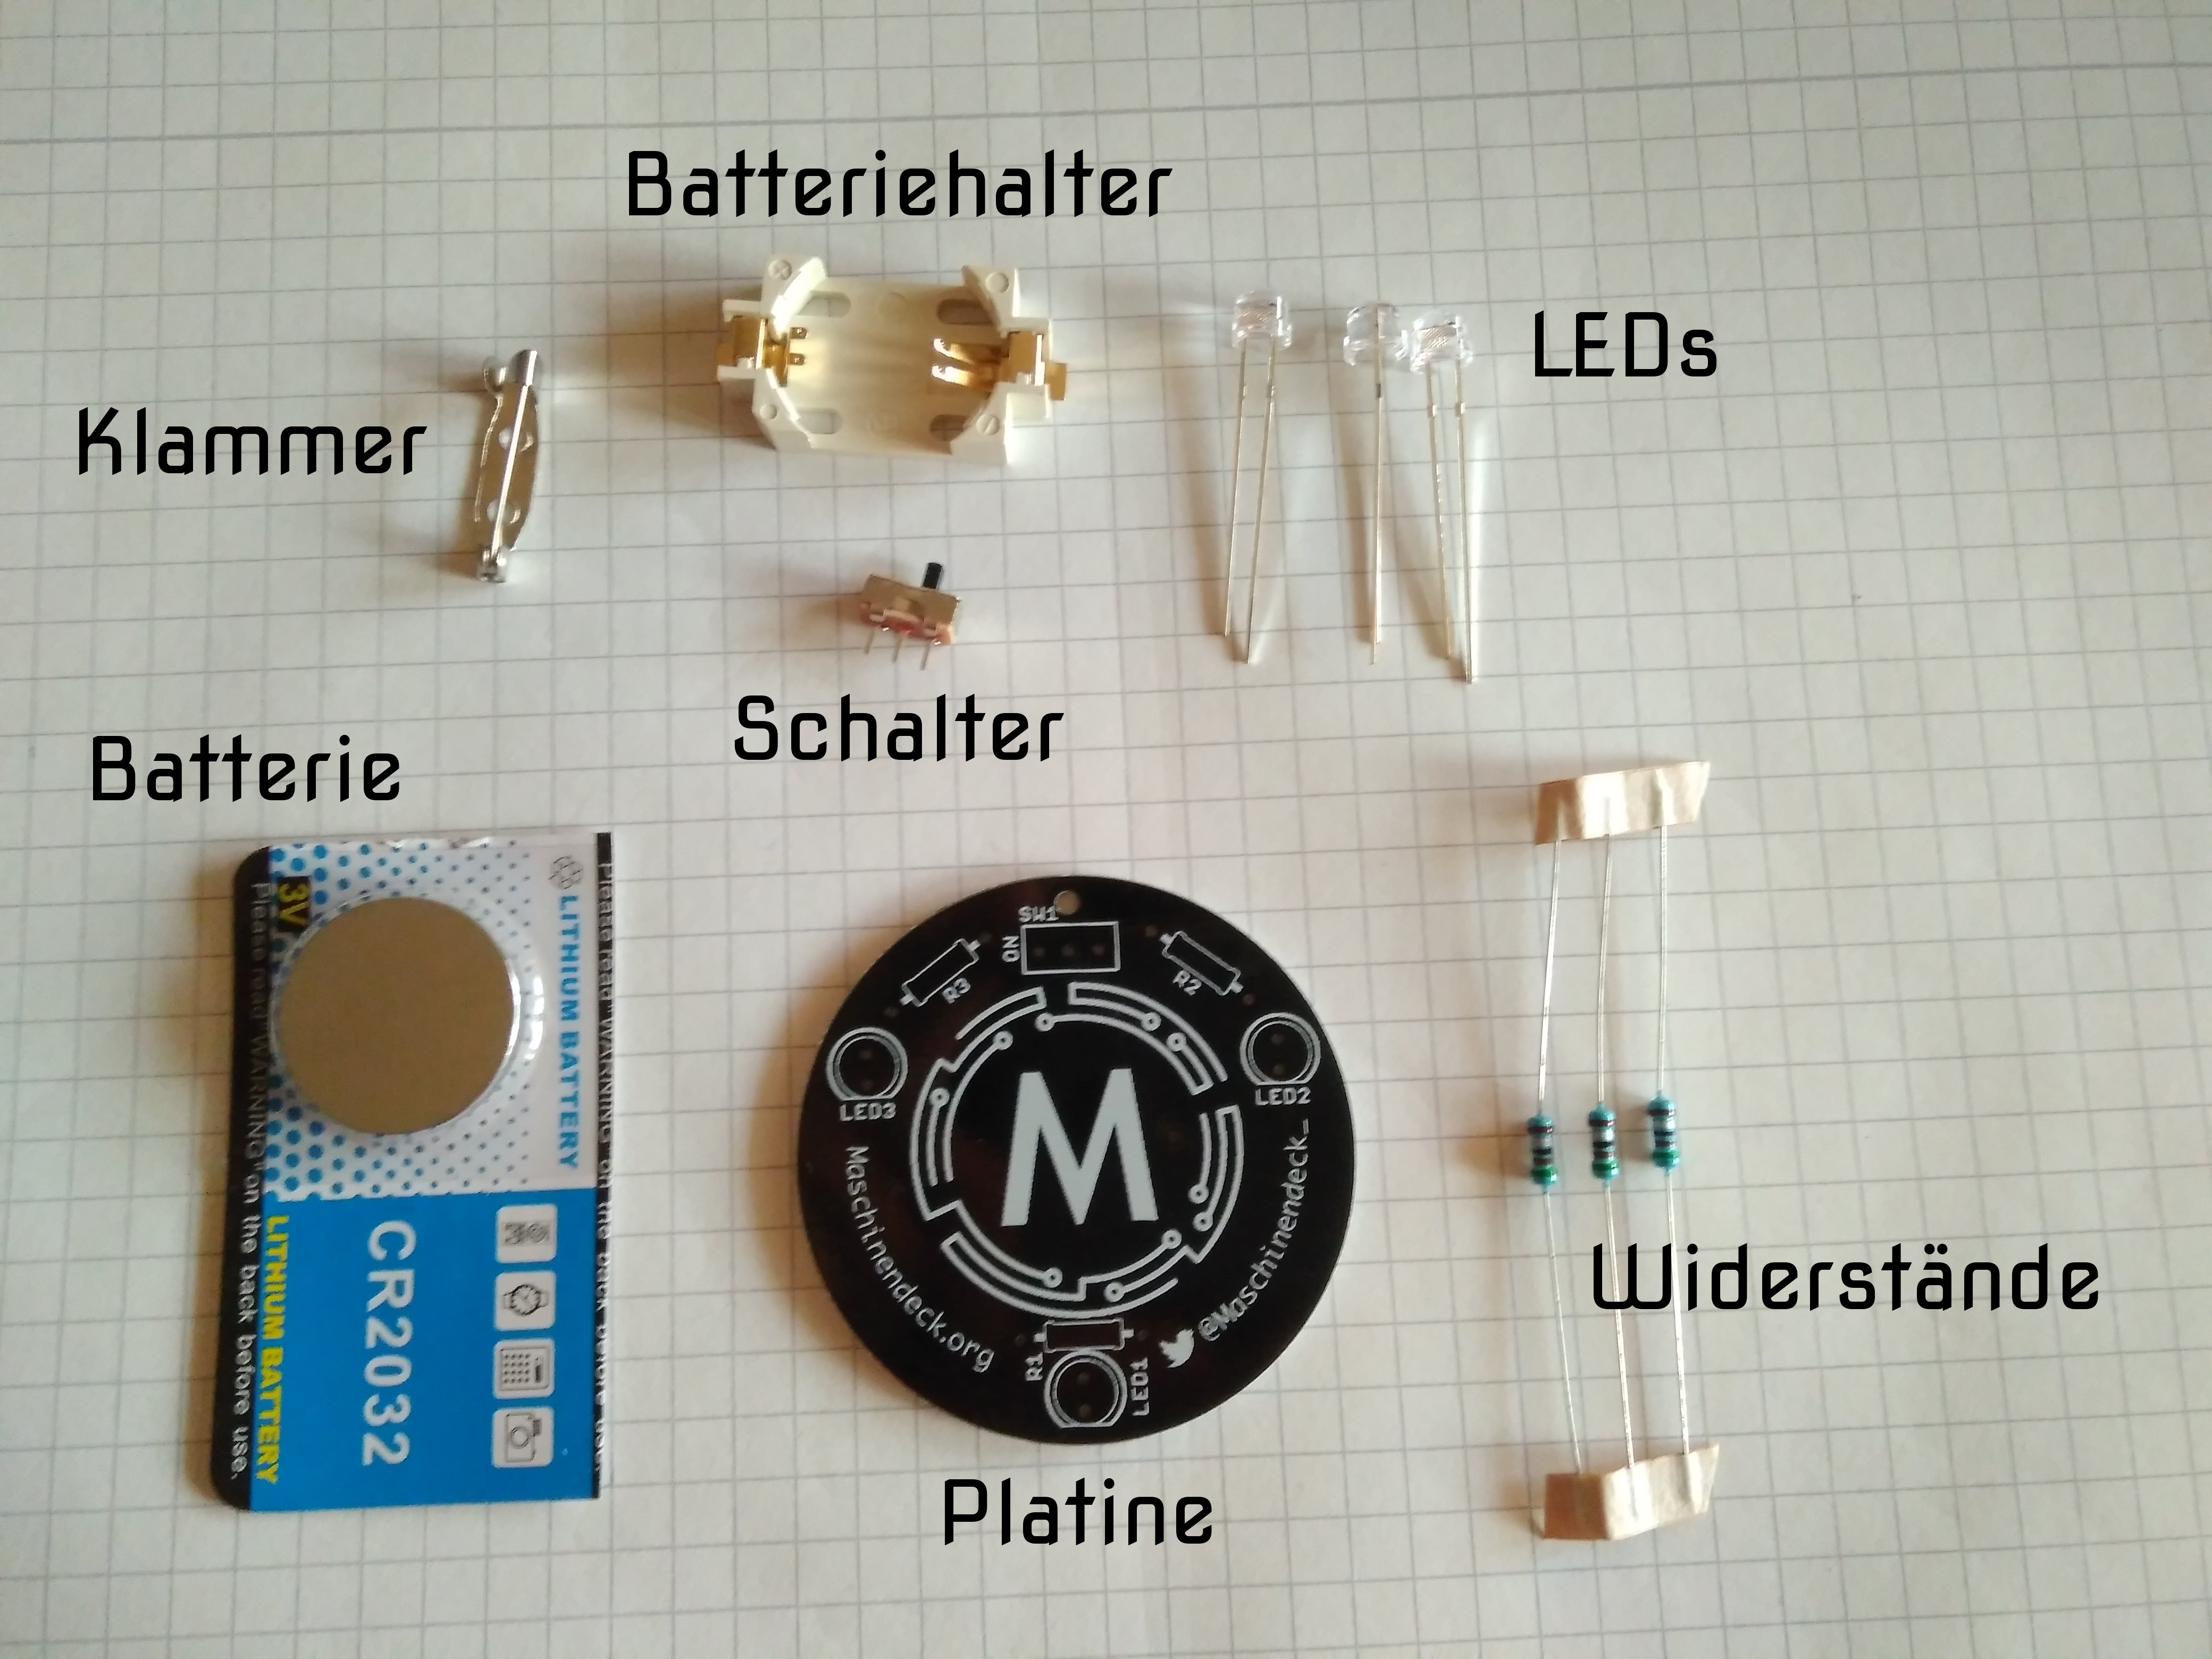
\includegraphics[width=\linewidth]{images/badge.jpg}
            \caption{Der Bausatz}
        \end{figure}
    \end{frame}

    
\end{document}
